\documentclass[]{article}
\usepackage[utf8]{inputenc}
\usepackage{pdfpages}
\usepackage{amsmath}
\usepackage{amssymb}
\usepackage{graphicx}
\usepackage{geometry}
\usepackage{enumitem}
\usepackage{amsthm}

\geometry{hmargin=2cm}

\title{Algèbre et géométrie 1}

\author{Patrick Le Meur et Pierre Gervais}

% Environnement type théorème
\newtheorem{mythm}{Théorème}
\newtheorem{myproposition}{Proposition}
\newtheorem{myproperty}{Propriété}
\newtheorem{mylemma}{Lemme}
\newtheorem{mycor}{Corollaire}

% Environnement type texte
\theoremstyle{remark}
\newtheorem{mynot}{Notation}
\newtheorem{myrem}{Remarque}
\newtheorem{myexer}{Exercice}
\newtheorem{myproof}{Preuve}
\newtheorem{myexmpl}{Exemple}

% Environnement de définition
\theoremstyle{definition}
\newtheorem{mydef}{Définition}

\setlist[itemize]{label=-}

% Carré de fin de preuve
\newcommand{\cqfd}{
	\hfill$\square$
}

% "Checkmark" de fin d'étape de preuve
\newcommand{\checked}{
	\hfill$\checkmark$
}

% Définition de fonction
\newcommand{\func}[5]{
#1 ~ : ~ \left\{ \begin{array}{lcl}
	#2 & \longrightarrow & #3 \\
	#4 & \longmapsto & #5
\end{array}
\right.
}

\newcommand{\funcinline}[5]{
#1 ~ : ~ #2 \longrightarrow #3, ~ #4 \longmapsto #5
}

\newcommand{\funcshort}[3]{
#1 ~ : ~ #2 \longrightarrow #3
}

\newenvironment{proofpart}[1]{
	\noindent
	{\boldmath #1}
}{
	\checkmark
}

\begin{document}
	\section{Introduction}
		On considère ici des endomorphismes linéaires d'un espace vectoriel de dimension fini, pour simplifier les choses on se contentera de l'espace $\mathbb{R}^n$.
		
		On notera $\mathcal{C}_n=(c_i)_{1 \leqslant i \leqslant n}$ la base canonique de $\mathbb{R}^n$.
		
		\paragraph{Présentation du changement de base :}
		
		commençons par une étude de cas simple.
		\begin{itemize}
			\item $f$ est la symétrie par rapport à l'axe des abscisses
			\item $b$ est la rotation d'angle $\frac{\pi}{4}$ composée à l'homothétie de rapport $\frac{\sqrt{2}}{2}$
		\end{itemize}
		
		
		Une application linéaire est définie par les valeurs qu'elle prend sur une base $e$.

		On commence avec $e=\mathcal{C}_n$.
		
		\begin{figure}[h!]
			\centering
			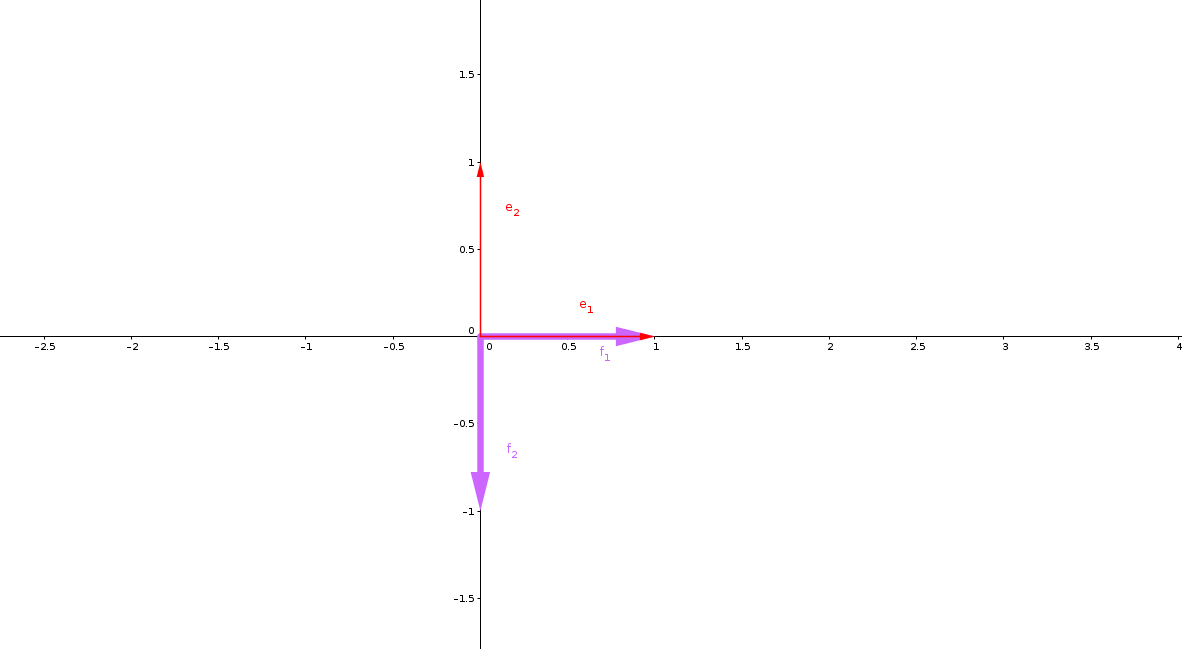
\includegraphics[width=350pt]{Img1.png}
			\caption{Image de la base canonique par $f$}
		\end{figure}

		On a choisi ici d'étudier l'image de la base canonique par $f$, mais que se serait-il passé si on avait choisi une autre base ?
		
		Prenons à présent $e_1=\binom{1}{1}$ et $e_2=\binom{-1}{1}$, c'est à dire $e_1=b(c_1)$ et $e_2=b(c_2)$.
		
		\newpage
		
		\begin{figure}[h!]
			\centering
			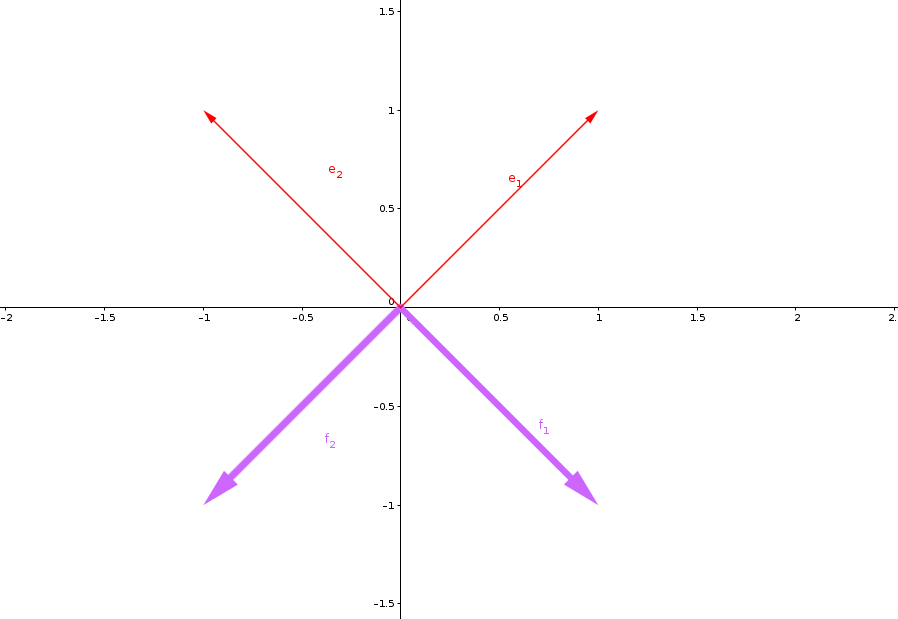
\includegraphics[width=350pt]{Img2.png}
			\caption{Image de la base $\left(\binom{1}{1},\binom{-1}{1}\right)$ par $f$}
		\end{figure}
		
		L'application $b$ envoie la base $\mathcal{C}_n$ sur la base $e$, alors pour tout $i=1, 2$ :
		
		$$b(c_i)=e_i$$
		
		$$(f \circ b)(c_i) = f(e_i) = \lambda_1 e_1 + \lambda_2 e_2$$
		
		Où $\lambda_1$ et $\lambda_2$ sont les coordonnées de $f(e_i)$ dans la base $e$.
		
		$$(f \circ b)(c_i) = \lambda_1 e_1 + \lambda_2 e_2 = \lambda_1 b (c_1) + \lambda_2 b (c_2)$$
		
		$$(b^{-1} \circ f \circ b)(c_i) = \lambda_1 c_1 + \lambda_2 c_2$$
		
		On a donc une nouvelle application $f_e = b^{-1} \circ f \circ b$ qui est telle que $f(c_i)$ a les même coordonnées dans la base $\mathcal{C}_n$ que $f(e_i)$ dans la base $e$.

		Cette manipulation permet d'écrire facilement la matrice représentative de $f$ dans la base $e$.

\section{Représentation matricielle d'une application linéaire}

	Soit $\varphi$ une application linéaire de $\mathbb{R}^n$ vers $\mathbb{R}^n$ et $e=(e_i)_i$ et $f=(f_i)_i$ deux bases de $\mathbb{R}^n$.
	
	Si pour tout $i=1, ..., n$ on a la décomposition de $f(e_i)$ dans la base $f$ :
	
	$$f(e_i) = \sum_{j=1}^{n} \varphi_{i,j} f_j$$

	On stocke ces valeurs $\varphi_{i,j}$ dans une matrice $M_{e,f}=(\varphi_{i,j})_{1 \leqslant i, j \leqslant n}$ qui détermine entièrement l'application $\varphi$ mais qui \textbf{dépend des bases de départ $e$ et d'arrivée $f$}.

	Dans le cas où $f=\mathcal{C}_n$, la décomposition de chaque vecteur $\mathcal{C}_n$ est simple :
	
	$$\varphi(x) = \left(\begin{array}{c}
		y_1 \\ y_2 \\ \vdots \\y_n
	\end{array}\right) = y_1 c_1 + y_2 c_2 + ... + y_n c_n$$
	
	La matrice de $\varphi$ dans les bases $e$ et $\mathcal{C}_n$ s'écrit alors $M_{e, \mathcal{C}_n} = (\varphi(e_1) ~ | ~ \varphi(e_2) ~ | ~ ... ~ | ~\varphi(e_n))$ où $ \cdot ~ | ~ \cdot$ est l'opération de juxtaposition de matrices (ici de vecteurs colonne).
	
\section{Changements de base}
	
	On considère toujours deux bases $e$ et $f$, une application linéaire $f$ de $\mathbb{R}^n$ et sa représentation matricielle $M$ dans ces bases. 
	
	Soit $g$ une autre base, on pose $E$ la matrice inversible qui envoie la base $e$ sur la base $g$, c'est à dire telle que $E e_i=g_i$ et $E^{-1} g_i=e_i$, et de même la matrice $F$ pour la base $f$ :

\begin{center}
	\begin{tabular}{|c|c|c|c|}
		\hline
		Base de départ & Base d'arrivée & Matrice & Explication \\
		\hline
		e & f & $M$ & $Me_i = \sum \lambda_j f_j$ \\
		g & f & $ME^{-1}$ & $ME^{-1}g_i=M e_i = \sum \lambda j f_j$ \\
		e & g & $FM$ & $FM e_i = \sum \lambda_j F f_j = \sum \lambda_j g_j$ \\
		g & g & $FME^{-1}$ & $FME^{-1} g_i = FMe_i = \sum \lambda_j F f_j = \sum \lambda_j g_j$ \\
		\hline
	\end{tabular}
\end{center}
	 
\end{document}
